\documentclass[	DIV=calc,%
							paper=a4,%
							fontsize=11pt,%
							twocolumn]{scrartcl}	 					% KOMA-article class

\usepackage{lipsum}													% Package to create dummy text

\usepackage[english]{babel}										% English language/hyphenation
\usepackage[protrusion=true,expansion=true]{microtype}				% Better typography
\usepackage{amsmath,amsfonts,amsthm}					% Math packages
\usepackage[pdftex]{graphicx}									% Enable pdflatex
\usepackage[svgnames]{xcolor}									% Enabling colors by their 'svgnames'
\usepackage[hang, small,labelfont=bf,up,textfont=it,up]{caption}	% Custom captions under/above floats
\usepackage{epstopdf}												% Converts .eps to .pdf
\usepackage{subfig}													% Subfigures
\usepackage{booktabs}												% Nicer tables
\usepackage{fix-cm}		
\usepackage{cleveref}
% various theorems, numbered by section

\newtheorem{thm}{Theorem}[section]
\newtheorem{lem}[thm]{Lemma}
\newtheorem{prop}[thm]{Proposition}
\newtheorem{cor}[thm]{Corollary}
\newtheorem{conj}[thm]{Conjecture}

\theoremstyle{definition}
\newtheorem{defn}[thm]{Definition}
\newtheorem{defns}[thm]{Definitions}
\newtheorem{con}[thm]{Construction}
\newtheorem{exmp}[thm]{Example}
\newtheorem{notn}[thm]{Notation}
\newtheorem{notns}[thm]{Notations}
\newtheorem{addm}[thm]{Addendum}
\newtheorem{exer}[thm]{Exercise}
\newtheorem{rem}[thm]{Remark}
\theoremstyle{plain}


\theoremstyle{remark}
\newtheorem{rems}[thm]{Remarks}
\newtheorem{warn}[thm]{Warning}
\newtheorem{sch}[thm]{Scholium}
\DeclareMathOperator{\id}{id}

\newcommand{\bd}[1]{\mathbf{#1}}  % for bolding symbols
\newcommand{\RR}{\mathbb{R}}      % for Real numbers
\newcommand{\ZZ}{\mathbb{Z}}      % for Integers
\newcommand{\col}[1]{\left[\begin{matrix} #1 \end{matrix} \right]}
\newcommand{\comb}[2]{\binom{#1^2 + #2^2}{#1+#2}}
%%% Custom sectioning (sectsty package)
\usepackage{sectsty}													% Custom sectioning (see below)
\allsectionsfont{%															% Change font of al section commands
	\usefont{OT1}{phv}{b}{n}%										% bch-b-n: CharterBT-Bold font
	}

\sectionfont{%																% Change font of \section command
	\usefont{OT1}{phv}{b}{n}%										% bch-b-n: CharterBT-Bold font
	}



%%% Headers and footers
\usepackage{fancyhdr}												% Needed to define custom headers/footers
	\pagestyle{fancy}														% Enabling the custom headers/footers
\usepackage{lastpage}	

% Header (empty)
\lhead{}
\chead{}
\rhead{}
% Footer (you may change this to your own needs)
\lfoot{\footnotesize \texttt{www.albohessab.weebly.com} \textbullet ~Miliyon T.}
\cfoot{}
\rfoot{\footnotesize page \thepage\ of \pageref{LastPage}}	% "Page 1 of 2"
\renewcommand{\headrulewidth}{0.0pt}
\renewcommand{\footrulewidth}{0.4pt}



%%% Creating an initial of the very first character of the content
\usepackage{lettrine}
\newcommand{\initial}[1]{%
     \lettrine[lines=3,lhang=0.3,nindent=0em]{
     				\color{DarkGoldenrod}
     				{\textsf{#1}}}{}}



%%% Title, author and date metadata
\usepackage{titling}															% For custom titles

\newcommand{\HorRule}{\color{DarkGoldenrod}%			% Creating a horizontal rule
									  	\rule{\linewidth}{1pt}%
										}

\pretitle{\vspace{-30pt} \begin{flushleft} \HorRule
				\fontsize{50}{50} \usefont{OT1}{phv}{b}{n} \color{DarkRed} \selectfont
				}
\title{My first triumph in Mathematics}					% Title of your article goes here
\posttitle{\par\end{flushleft}\vskip 0.5em}

\preauthor{\begin{flushleft}
					\large \lineskip 0.5em \usefont{OT1}{phv}{b}{sl} \color{DarkRed}}
\author{Miliyon T., }											% Author name goes here
\postauthor{\footnotesize \usefont{OT1}{phv}{m}{sl} \color{Black}
					Addis Ababa University 							% Institution of author
					\par\end{flushleft}\HorRule}

\date{September 7, 2014}																				% No date



%%% Begin document
\begin{document}

\maketitle
\thispagestyle{fancy} 			% Enabling the custom headers/footers for the first page
% The first character should be within \initial{}
\initial{M}\textbf{y first triumph in mathematics was Steiner triple problem. While I was in AAU, my professor Dr. Yirgalem introduce me the problem. She thought it was "open". It took me a day to solve it. But I doubted that it might have been solved already. So, I searched on the internet. My instinct was correct. It has been solved by Kirkman.\footnote{The British mathematician Thomas Kirkman(1806 - 1895) solved the problem in his $1847$ paper.}}

\section{Definition}
\begin{defn}[Graph] A Graph is a non empty set of vertices and edges. It is often denoted
\begin{align*}
G=(V,E) \text{ or } (V_G,E_G) \text{ or } (V(G),E(G))
\end{align*}
\end{defn}

\begin{figure}[hbt!]
\centering
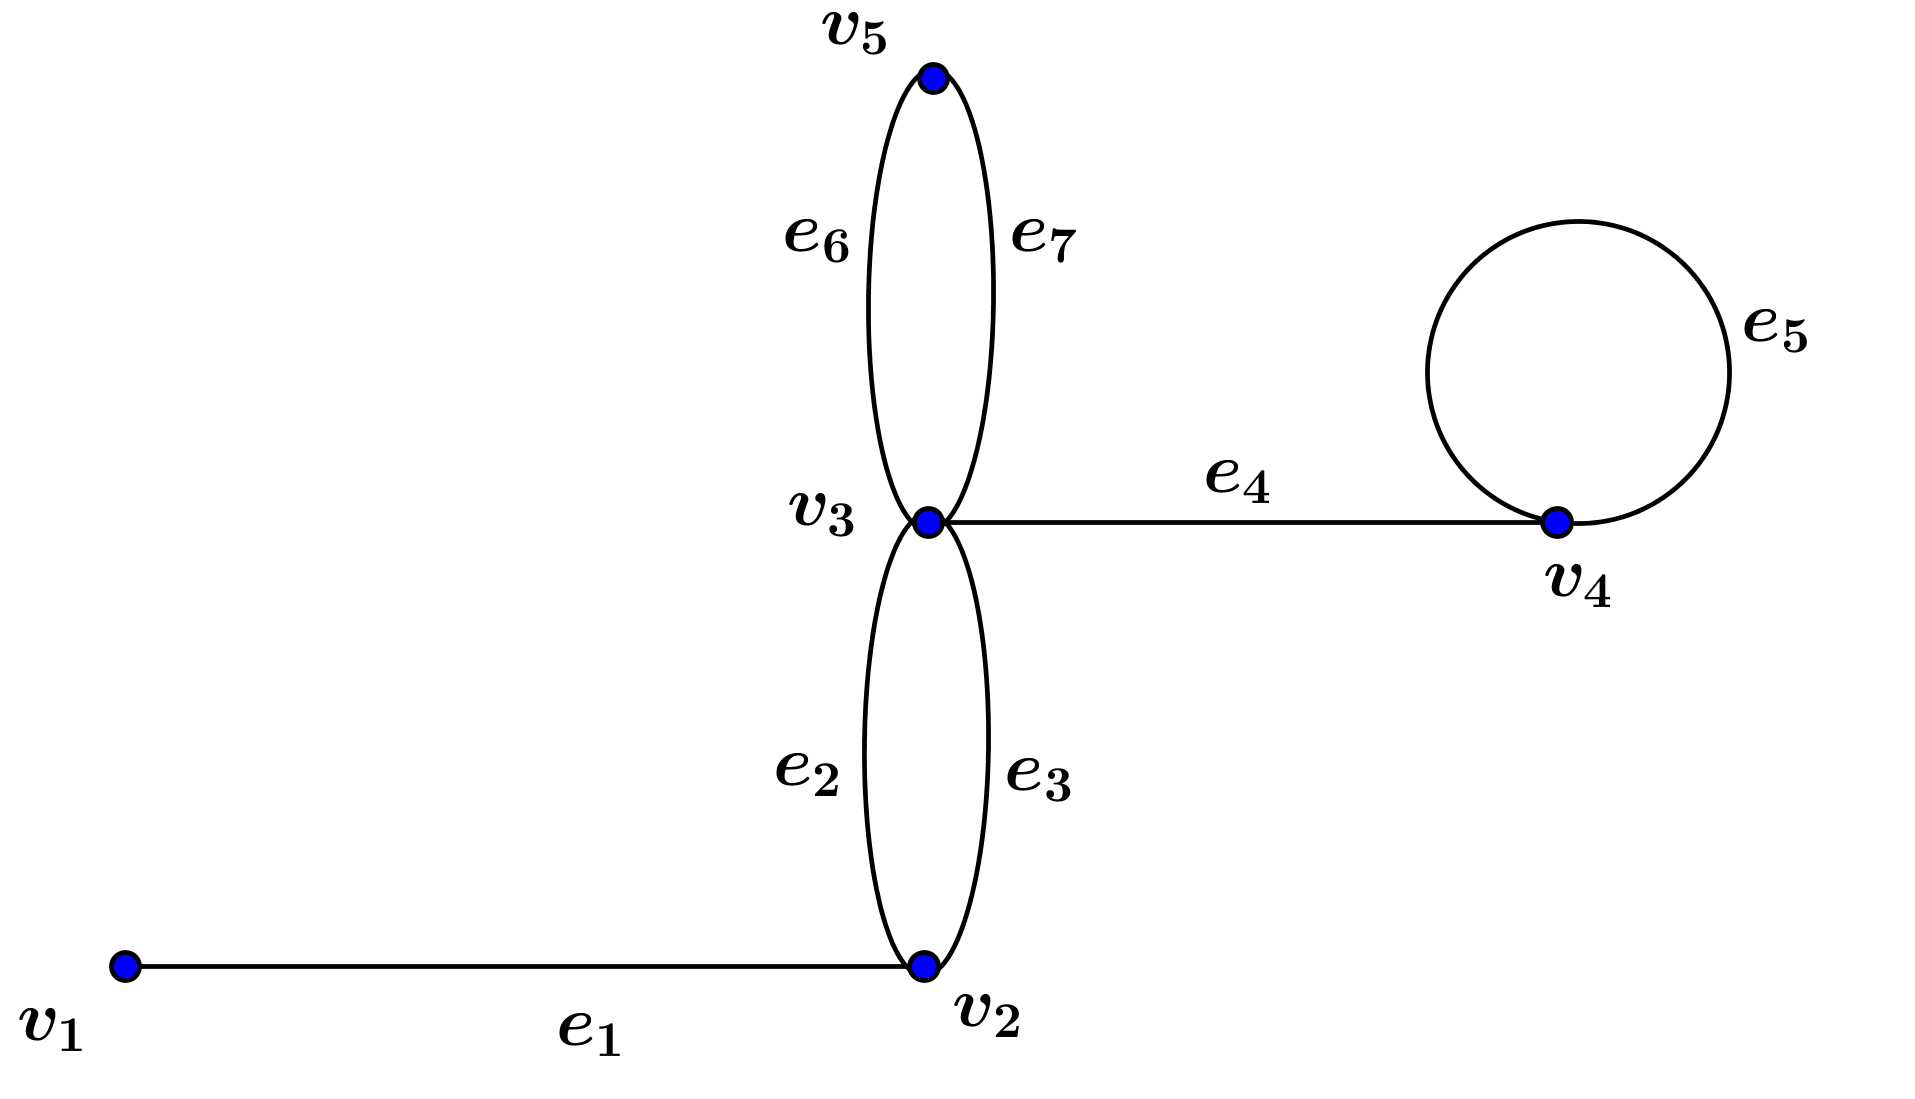
\includegraphics[width=.4\textwidth]{graph.png}
\caption{A Graph}\label{fig1}
\end{figure}

\begin{defn}[Vertex]
A point; an element of the first constituent set of a graph.
\end{defn}
\begin{defn}[Degree (of a vertex)]
Given a vertex $v$,the number $deg(v)$ of instances of $v$ as an endpoint; that is, the number of proper edges incident on $v$ plus twice the number of loops at $v$.
\end{defn}

\begin{defn}[Order]
Given a graph $G$, the cardinality $|V_G|$ of the vertex set. It is denoted by $|G|$.
\end{defn}

\begin{defn}[Link]
An edge with two distinct end point.
\end{defn}

\begin{exmp}
The edge $e_1$ in (\textbf{Figure} \ref{fig1}) is a link.
\end{exmp}

\begin{defn}[Loop]
An edge joining a vertex to itself.
\end{defn}

\begin{exmp}
The edge $e_5$ in (\textbf{Figure} \ref{fig1}) is a loop.
\end{exmp}

\begin{defn}[Multi-edge]
 A set of at least two edges,all of which have the same endpoints.
\end{defn}
\begin{defn}[Simple Graph]
A graph with no loops or multi-edge.
\end{defn}
\begin{figure}[hbt!]
\centering
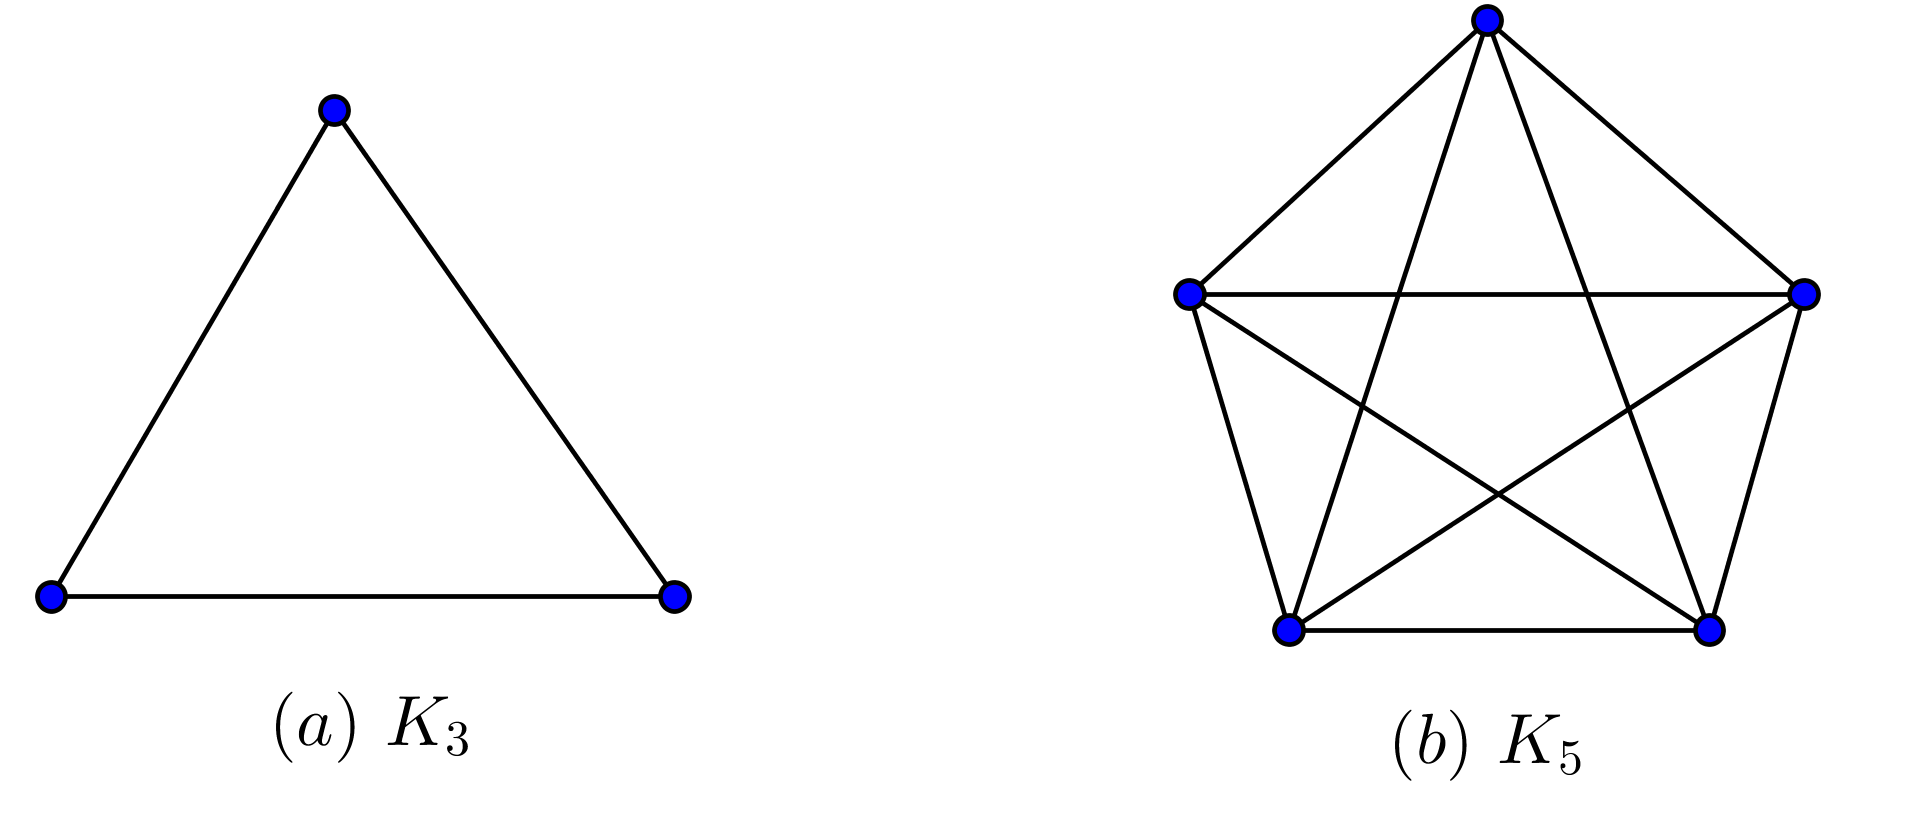
\includegraphics[width=.5\textwidth]{simplegraph.png}
\caption{A Simple Graph}\label{fig2}
\end{figure}

\begin{defn}[Edge]
A line,either joining one vertex to another or joining a vertex to itself; an element of the second constituent set of a graph.
\end{defn}

\begin{defn}[Size]
Given a graph $G$, the cardinality $|E_G|$ of the edge set. It is denoted by $||G||$.
\end{defn}

\begin{defn}[Subgraph]
Given a graph $G$,a graph $H$ whose vertices and edges are all in $G$.
\end{defn}

\begin{defn}[Walk]
An alternating sequence $v_0, e_1, v_1,...,e_r, v_r$ of vertices and edges where consecutive edges are adjacent,so that each edge $e_i$ joins vertices $v_{i−1}$ and $v_i$.
\end{defn}

\begin{defn}[Trial]
A \textit{walk} in which no edge occurs more than once.
\end{defn}

\begin{defn}[Path]
A \textit{trail} in which all of its vertices are different, except that the initial and final vertices may be the same.
\end{defn}

\begin{defn}[Cycle]
A closed \textit{path} of positive length.
\end{defn}

\begin{defn}
The simple graph $K_n$ with n vertices in which every pair of vertices is adjacent.
\end{defn}

\begin{figure}[hbt!]
\centering
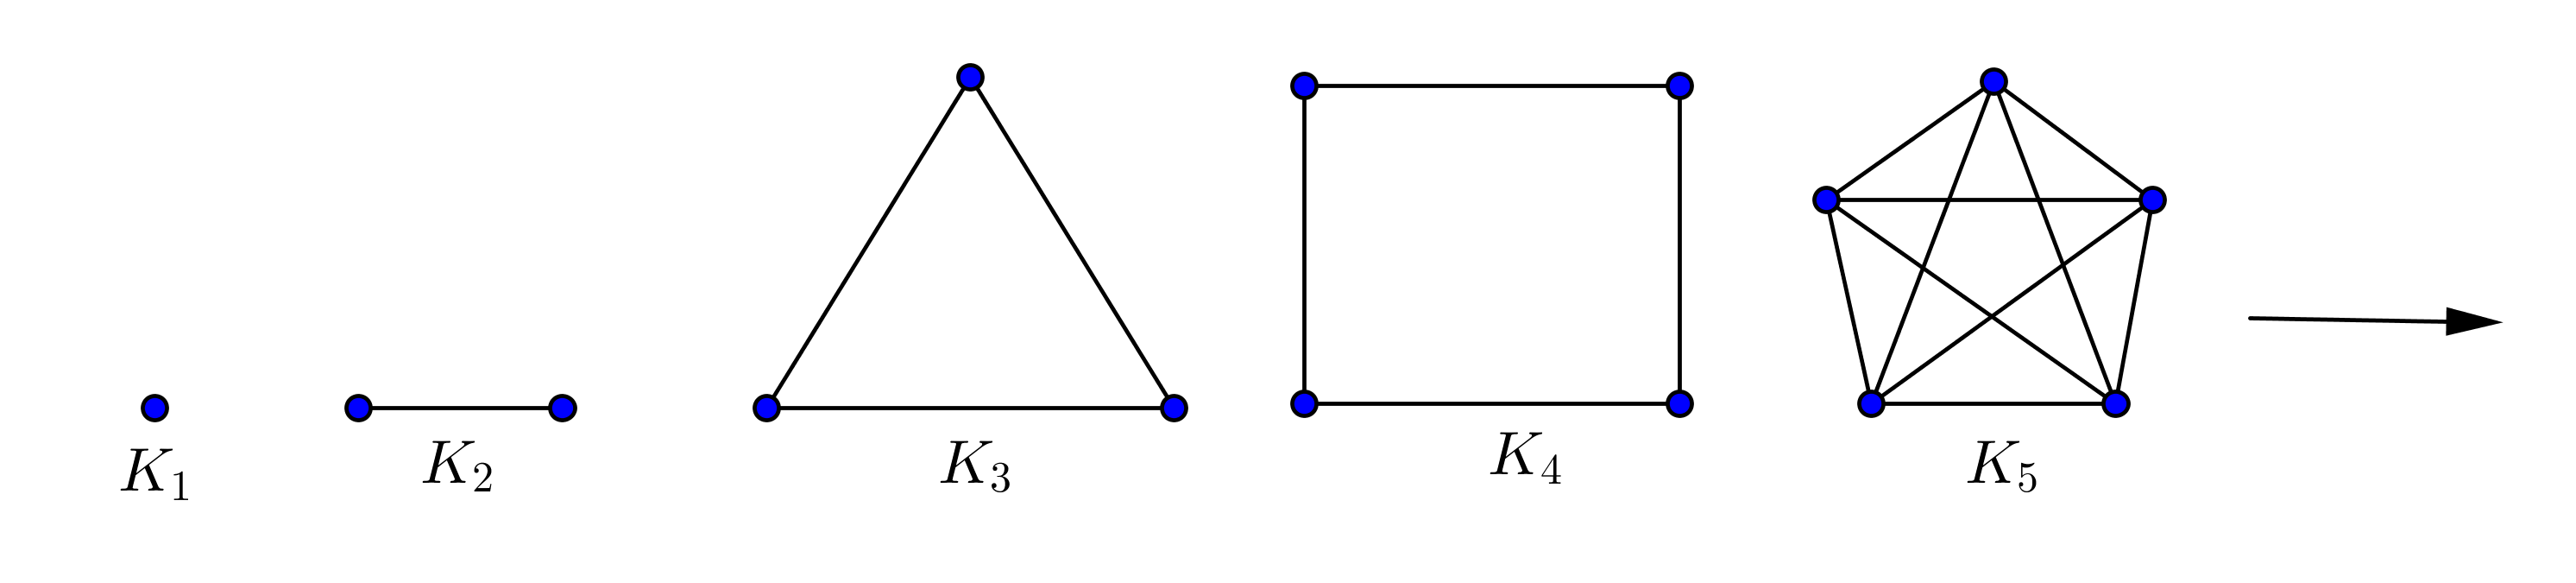
\includegraphics[width=.5\textwidth]{completegraph.png}
\caption{Complete graph}\label{fig3}
\end{figure}

\begin{defn}[Decomposition] A decomposition od a graph $G$ is a family $\mathcal{F}$ of edge-disjoint subgraph of $G$ such that $$ \bigcup_{F\in \mathcal{F}}E(F) = E(G)$$

\end{defn}

\begin{defn}[Cyclic Decomposition]
If every subgraph of $\mathcal{F}$ is a cycle, then the decomposition is called cyclic decomposition.
\end{defn}

\section{Basic Results}

\begin{thm}(Handshaking lemma)
For any graph $G$
\begin{align}
\sum_{v\in V(G)}deg(v)=2||G||
\end{align}
\end{thm}

\begin{proof}
When summing the degrees of the vertices of a graph $G$, we count each edge of $G$ twice, once for each of the two vertices incident with the edge.
\end{proof}

\begin{cor}
The number of odd vertices(Vertices of odd degree) in a graph is even
\end{cor}

\begin{proof}
Let $G$ be any graph. Partition the vertex set $V(G)$ into two
\begin{align*}
O&- \text{the set of all odd vertices}\\
E&-\text{the set of all odd vertices}
\end{align*}
Then we have
\begin{align}
\sum_{v\in V(G)}deg(v)=\sum_{v\in O}deg(v) + \underbrace{\sum_{v\in E}deg(v)}_{even}
\end{align}
Now, suppose the number of odd vertices in $G$ is odd. Hence the sum 
\begin{align*}
\sum_{v\in O}deg(v)\text{ is odd.}
\end{align*}
Consequently, the sum 
\begin{align*}
\sum_{v\in V(G)}deg(v)\text{ becomes odd.}
\end{align*}
That is a contradiction to Handshaking lemma. Therefore the number of odd vertices in any graph $G$ must be even.
\end{proof}
\begin{cor}
The size of a complete graph of order $n$ ($K_n$) is
\begin{align}
\binom{n}{2}=\frac{n(n-1)}{2}
\end{align} 
\end{cor}

\section{Triumph}

\begin{lem}
$K_n$ can be decomposed into cycles of $m$ iff $||K_n||$ is a multiple of $m$.
\end{lem}

\begin{proof}

\end{proof}


\begin{thm}
If $K_n$ decomposes into $K_3$ (Cycles of order $3$), then either $n=6q+1$ or $n=6q+3$ for some integer $q$.
\end{thm}

\begin{proof}

\end{proof}

\begin{thebibliography}{9}

\bibitem{May}
[Adrian Bondy \& Murty] ~
Graph Theory, 2007.


\bibitem{amsshort}
[Gary Chartrand]  ~
Introductory Graph Theory.

\bibitem{Jun}
[Charles \& Jeffrey]~
Handbook of combinatorial design.
\end{thebibliography}
\end{document}
